\section{K-means 聚类}

\begin{definition}[聚类分析]
    聚类分析是一种将数据集划分为多个簇（Cluster）的技术，使得同一簇内的数据点相似度较高，而不同簇之间的数据点相似度较低。聚类分析常用于探索性数据分析、图像处理、市场细分等领域。
\end{definition}

\begin{definition}[无监督问题与有监督问题]
    当我们手里对一组数据没有标签时，称为无监督问题。事先无法对样本进行准确的判定，需要建立和总结一定的规则模式后再定性的，属于无监督学习。相反，样本一开始就拥有“目标”标签的话，我们所进行的从特征到目标的建模，则是有监督的学习。
\end{definition}

\begin{definition}[K-Means 算法]
    K-Means 算法预先指定初始聚类数以及初始化聚类中心，按照样本之间的距离大小，把样本集根据数据对象与聚类中心之间的相似度划分为类簇，不断更新聚类中心的位置，不断降低类簇的误差平方和（Sum of Squared Error，SSE），当 SSE 不再变化或目标函数收敛时，聚类结束，得到最终结果。

    \begin{enumerate}
        \item 先从数据集中随机选取K个初始聚类中心 $\mathrm{C_i}(1 \leq \mathrm{i} \leq \mathrm{k})$ ，计算其余数据对象与聚类中心 $C_i$ 的欧氏距离，找出离目标数据对象最近的聚类中心 $C_i$ ，并将数据对象分配到聚类中心 $C_i$ 所对应的簇中；
        \item 接着计算每个簇中数据对象的平均值，将该值当作新的聚类中心，进行下一次迭代，直到聚类中心不再变化或达到最大的迭代次数时停止。
    \end{enumerate}

    空间中数据对象与聚类中心间的欧氏距离计算公式为：
    $$
        d\left(X, C_i\right)=\sqrt{\sum_{j=1}^m\left(X_j-C_{i j}\right)^2}
    $$
    其中，$X$ 为数据对象；$C_i$ 为第 $i$ 个聚类中心；$m$ 为数据对象的维度；$X_j 、 C_{ij}$ 为 $X$ 和 $C_i$ 的第 $j$ 个属性值。

    整个数据集的 SSE 计算公式为：
    $$
        \mathrm{SSE}=\sum_{i=1}^k \sum_{X \in C_i}\left|d\left(X, C_i\right)\right|^2
    $$
    其中，SSE 的大小表示聚类结果的好坏；$k$ 为簇的个数。
\end{definition}

\begin{figure} [H]
    \centering
    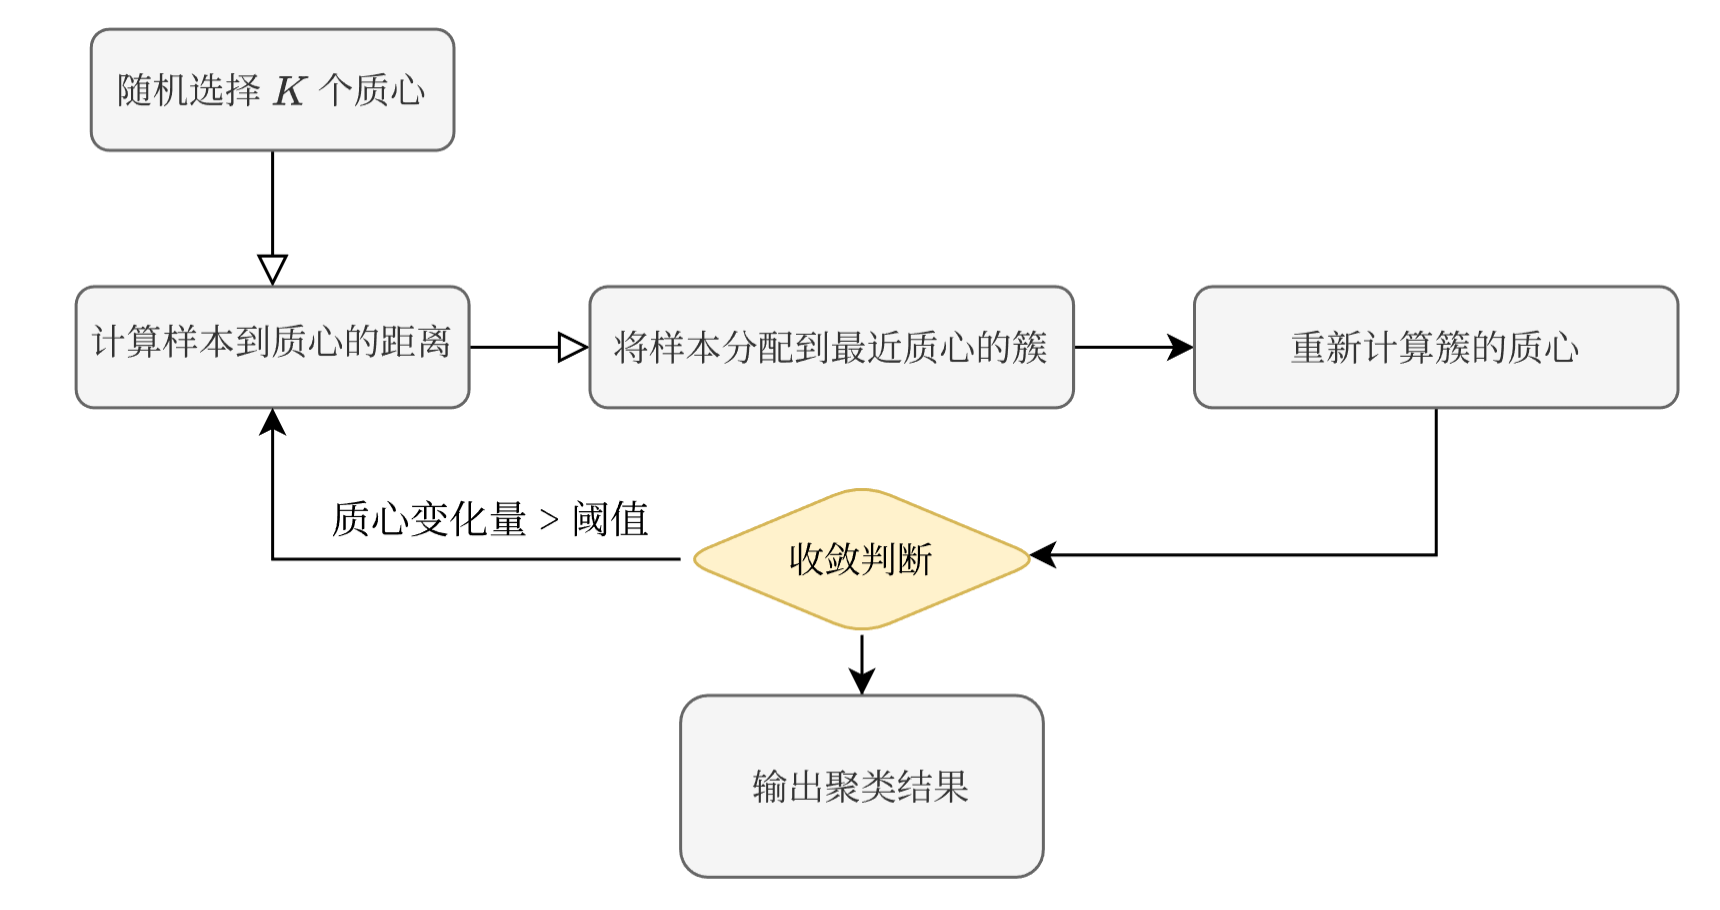
\includegraphics[width=0.5\textwidth]{chapters/聚类分析/images/K-means/kmeans-drawio.png}
\end{figure}

K-Means 的本质是通过迭代最小化 SSE 实现聚类，默认距离使用欧氏距离。但也可以根据数据类型替换为：

\begin{definition}[曼哈顿距离]
    （适用于高维稀疏数据）
    $$\sum\left|x_i-y_i\right|$$
\end{definition}

\begin{definition}[余弦相似度]
    夹角越大，余弦值越小，相似度越低：
    $$
        \text { similarity }=\cos (\theta)=\frac{A \cdot B}{\|A\|\|B\|}=\frac{\sum_{i=1}^n A_i B_i}{\sqrt{\sum_{i=1}^n A_i^2} \sqrt{\sum_{i=1}^n B_i^2}}
    $$
    由于 $cos \in [-1,1]$ ，它判断的是向量之间的方向而不是大小；两个向量有同样的方向那么 $\cos$ 相似度为$1$，两个向量方向相对成 $90^\circ$ 那么 $\cos$ 相似度为$0$，两个向量正相反那么 $\cos$ 相似度为$-1$，和它们的大小无关。

    当向量的方向比其大小更重要时，就要考虑使用余弦相似度。因为欧几里得距离衡量的是空间中两点之间的绝对直线距离。
\end{definition}

\begin{example}
    在文本挖掘中与文档聚类中，一篇文章通常被表示成一个高维的词频向量（例如 TF-IDF 向量），向量的每个维度代表一个词，维度的值代表该词的重要性。
\end{example}

\begin{solution}
    \begin{enumerate}
        \item 欧几里得距离的问题: 由于长文的词频值普遍更高，它的向量长度会远大于短文的向量。如果我们用欧几里得距离，算法会认为这两篇文章“相距甚远”，因为它们的向量大小差异巨大。
        \item 余弦相似度的优势: 余弦相似度忽略了文章的长度（总词频），只关注词频的分布比例和方向。因为两篇文章都在讨论“机器学习”，它们在“模型”、“训练”、“数据”等词的维度上都有较高的值，所以它们的向量方向会非常接近。余弦相似度会正确地判断出这两篇文章在主题上是高度相似的，应该被聚在同一类。
    \end{enumerate}
\end{solution}

\begin{example}
    另一种常用的地方是推荐系统和用户画像上的聚类：
    \begin{enumerate}
        \item 用户A（一个苛刻的评分者）给电影《星际穿越》和《盗梦空间》分别评了 2 星和 1 星。
        \item 用户B（一个宽容的评分者）给这两部电影分别评了 5 星和 2.5 星。
    \end{enumerate}
\end{example}

\begin{solution}
    \begin{enumerate}
        \item 欧几里得距离的问题: 从数值上看，A(2, 1) 和 B(5, 2.5) 相差很大，欧式距离会认为他们是不同类型的用户。
        \item 余弦相似度的优势: 余弦相似度会发现，虽然B的评分普遍更高，但两个用户的评分模式（方向）是完全一样的：他们都认为《星际穿越》的好看程度是《盗梦空间》的两倍。这说明他们的品味是相似的。余弦相似度能够捕捉到这种“品味”上的一致性，而忽略评分“热情度”（大小）的差异。
    \end{enumerate}
\end{solution}

\subsection{余弦相似度求解}

在 K-Means 聚类中使用余弦距离 Cos Distance：\href{https://zhuanlan.zhihu.com/p/380389927}{https://zhuanlan.zhihu.com/p/380389927}

\begin{lstlisting}[style=python]
from sklearn.metrics.pairwise import cosine_similarity

def custom_distance(x1, x2):
    # Calculate the cosine similarity between x1 and x2
    similarity = cosine_similarity([x1], [x2])
    distance = 1 - similarity[0][0]
    return distance

    from sklearn.cluster import KMeans

# Create an instance of the KMeans class with our custom distance function
kmeans = KMeans(n_clusters=3, metric=custom_distance)
\end{lstlisting}

\subsection{K-Means 算法的缺陷}

K-Means 算法非常简单且使用广泛，但是主要存在以下 4 个缺陷。
\begin{enumerate}
    \item K 值需要预先给定，属于预先知识，很多情况下 K 值的估计是非常困难的，对于像计算全部微信用户的交往圈这样的场景就完全没办法用 K-Means 算法进行。对于可以确定K值不会太大但不明确精确的 K 值的场景，可以进行迭代运算，然后找出对应的 K 值，这个值往往能较好地描述有多少个簇类；
    \item K-Means 算法对初始选取的聚类中心点是敏感的，不同的随机种子点得到的聚类结果完全不同；
    \item K-Means 算法并不适合所有的数据类型。它不能处理非球形簇、不同尺寸和不同密度的簇；
    \item 易陷入局部最优解。
\end{enumerate}

\subsection{单位超球面聚类}

\begin{definition}[Hypersphere]

\end{definition}

\begin{figure} [H]
    \centering
    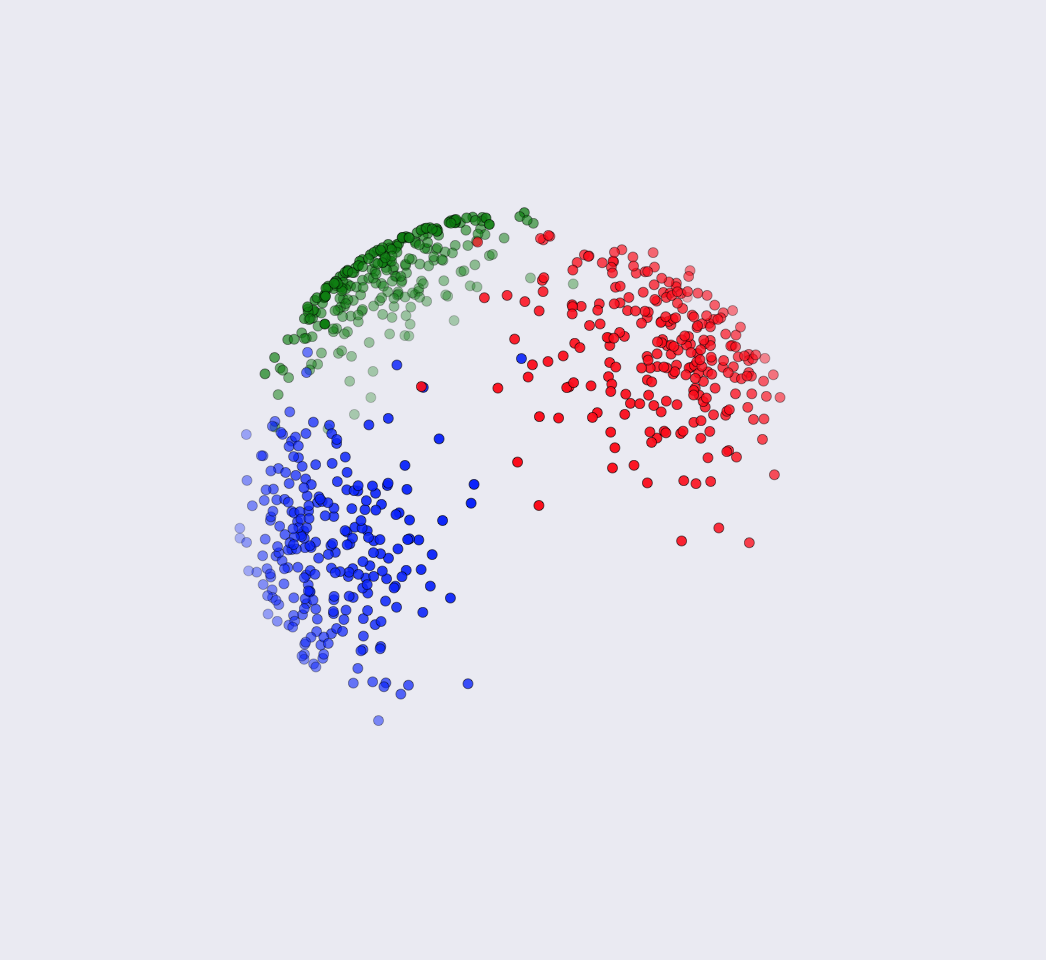
\includegraphics[width=0.4\textwidth]{chapters/聚类分析/images/K-means/img-20250901132604.png}
\end{figure}

参考：\href{https://github.com/jasonlaska/spherecluster}{https://github.com/jasonlaska/spherecluster}

\subsection{欧氏距离 Python 代码}

\begin{lstlisting}[style=python]
distortions = []
K_range = range(1, 10)
for k in K_range:
    model = KMeans(n_clusters=k,init='k-means++',n_init='auto',max_iter=300,tol=1e-4,random_state=0).fit(X)
    distortions.append(model.inertia_)  # inertia_ 属性直接给出了簇内平方和
\end{lstlisting}

掌握API参数是模型效果的关键保障：

\begin{center}
    \begin{tabular}{|l|l|l|l|}
        \hline 参数          & 默认值              & 说明      & 调优建议                  \\
        \hline n\_clusters & 8                & 聚类簇数K   & 通过肘部法则确定              \\
        \hline init        & 'k\_means++'     & 初始化方法   & 优先选'k\_means++'避免局部最优 \\
        \hline n\_init     & 10               & 不同初始化次数 & 增大值提升稳定性，但增加计算量       \\
        \hline max\_iter   & 300              & 最大迭代次数  & 高维数据建议增加到500          \\
        \hline tol         & $1 \mathrm{e}-4$ & 收敛阈值    & 值越小精度越高但可能不收敛         \\
        \hline algorithm   & 'auto'           & 算法实现    & 大数据选'elkan'提升速度       \\
        \hline
    \end{tabular}
\end{center}

\subsection{文本聚类的自定义距离函数}

\begin{example}
    当我们想要根据语义相似性对一组文本文档进行聚类。在这种情况下，欧氏距离可能不合适，因为它无法捕捉文档的语义含义。我们可以定义一个自定义距离函数，使用预先训练好的词向量模型（例如 Word2Vec 或 GloVe）来计算两个文档之间的语义相似度。
\end{example}

在下面的示例代码中，我们通过加载一个预先训练好的 Word2Vec 模型，并且自定义了一个距离函数，该函数使用模型将输入文档转换为词向量。

然后我们根据词向量计算词语之间的相似度，并采用余弦距离来聚类。

\begin{lstlisting}[style=python]
from gensim.models import Word2Vec

# Load the pre-trained Word2Vec model
model = Word2Vec.load("word2vec_model.bin")

def custom_distance(doc1, doc2):
    # Convert the documents to word vectors
    vec1 = [model[word] for word in doc1.split() if word in model]
    vec2 = [model[word] for word in doc2.split() if word in model]
    
    # Calculate the cosine similarity between the word vectors
    similarity = cosine_similarity(vec1, vec2)
    distance = 1 - similarity[0][0]
    return distance

from sklearn.cluster import KMeans

# Create an instance of the KMeans class with our custom distance function
kmeans = KMeans(n_clusters=5, metric=custom_distance)

# Fit the K-means model to the data
kmeans.fit(data)
\end{lstlisting}

